\documentclass[aspectratio=169,11pt]{beamer}
% docs/slides/preamble.tex -- 五份 deck 共享
\documentclass[aspectratio=169,11pt]{beamer}

% ==== 中文与字体 ====
\usepackage[UTF8,fontset=none]{ctex}
\usepackage{fontspec}

\IfFontExistsTF{PingFang SC}{%
  \setCJKmainfont{PingFang SC}[BoldFont=PingFang SC,ItalicFont=PingFang SC,AutoFakeSlant=0.15]
  \setCJKsansfont{PingFang SC}[ItalicFont=PingFang SC,AutoFakeSlant=0.15]
  \setCJKmonofont{PingFang SC}
}{%
  \IfFontExistsTF{Source Han Sans SC}{%
    \setCJKmainfont{Source Han Sans SC}
    \setCJKsansfont{Source Han Sans SC}
  }{%
    \IfFontExistsTF{Noto Sans CJK SC}{%
      \setCJKmainfont{Noto Sans CJK SC}
      \setCJKsansfont{Noto Sans CJK SC}
    }{%
      \setCJKmainfont{Heiti SC}
      \setCJKsansfont{Heiti SC}
    }
  }
}

\IfFontExistsTF{Helvetica Neue}{\setmainfont{Helvetica Neue}}{%
  \IfFontExistsTF{Inter}{\setmainfont{Inter}}{}}
\IfFontExistsTF{JetBrains Mono}{\setmonofont{JetBrains Mono}[Scale=0.85]}%
  {\setmonofont{Menlo}[Scale=0.85]}

% ==== 颜色 ====
\usepackage{xcolor}
\definecolor{cMain}{HTML}{1F4E79}
\definecolor{cAccent}{HTML}{E07A1F}
\definecolor{cGray}{HTML}{595959}
\definecolor{cMute}{HTML}{F4F4F4}
\definecolor{cOK}{HTML}{2E7D32}
\definecolor{cBad}{HTML}{B23A3A}
\definecolor{cWarn}{HTML}{C8A300}

% ==== 主题 ====
\usepackage{tcolorbox}
\usetheme{metropolis}
\metroset{progressbar=frametitle,numbering=fraction,block=fill}
\setbeamercolor{frametitle}{bg=cMain,fg=white}
\setbeamercolor{progress bar}{fg=cAccent,bg=cMute}
\setbeamercolor{alerted text}{fg=cAccent}
\setbeamercolor{title}{fg=cMain}

% metropolis 默认尝试 Fira Sans，未安装时 fallback 到 Latin Modern Sans。
% 这里在主题加载后显式覆盖，强制使用 macOS 上一定存在的 Helvetica Neue，
% 跟中文 PingFang 风格一致；找不到则按顺序尝试 Inter / Arial。
\IfFontExistsTF{Helvetica Neue}{%
  \setsansfont{Helvetica Neue}%
}{%
  \IfFontExistsTF{Inter}{\setsansfont{Inter}}{%
    \IfFontExistsTF{Arial}{\setsansfont{Arial}}{}}%
}

% ==== TikZ ====
\usepackage{tikz}
\usetikzlibrary{positioning,arrows.meta,fit,shapes.geometric,calc,%
  decorations.pathmorphing,backgrounds}

\tikzset{
  node-box/.style={draw=cMain,thick,rounded corners=2pt,
    minimum height=8mm,minimum width=18mm,align=center,font=\small},
  node-state/.style={draw=cMain,thick,circle,minimum size=14mm,
    align=center,font=\small},
  node-ok/.style={draw=cOK,thick,fill=cOK!10},
  node-warn/.style={draw=cWarn,thick,fill=cWarn!15},
  node-bad/.style={draw=cBad,thick,fill=cBad!10},
  % 色盲友好的状态机三态：蓝 (正常/Closed) / 橙 (告警/Open) / 灰 (中间/HalfOpen)
  % 避免 red-green 二元区分，改用 hue + lightness 双通道。
  node-state-normal/.style={draw=cMain,thick,fill=cMain!12},
  node-state-alert/.style={draw=cAccent,thick,fill=cAccent!18},
  node-state-transition/.style={draw=cGray,thick,fill=cGray!18},
  arrow/.style={-{Stealth[length=2mm]},thick,draw=cMain},
  arrow-async/.style={-{Stealth[length=2mm]},thick,dashed,draw=cGray},
  arrow-bad/.style={-{Stealth[length=2mm]},thick,draw=cBad},
  arrow-alert/.style={-{Stealth[length=2mm]},thick,draw=cAccent},
  lifeline/.style={dashed,thick,draw=cGray},
}

% ==== 代码 ====
\usepackage{listings}
\lstdefinelanguage{Go}{
  morekeywords={break,case,chan,const,continue,default,defer,else,
    fallthrough,for,func,go,goto,if,import,interface,map,package,range,
    return,select,struct,switch,type,var,nil,true,false,iota},
  morekeywords=[2]{string,int,int64,uint,uint64,bool,byte,error,context},
  sensitive=true,
  morecomment=[l]//,morecomment=[s]{/*}{*/},
  morestring=[b]",morestring=[b]`,
}
\lstdefinelanguage{LuaRedis}{
  morekeywords={and,break,do,else,elseif,end,false,for,function,if,in,
    local,nil,not,or,repeat,return,then,true,until,while},
  morekeywords=[2]{redis,call,KEYS,ARGV,tonumber,HGET,HSET,GET,SET,
    DECR,DECRBY,INCR,INCRBY,EXPIRE,PEXPIRE,ZADD,ZCARD,ZREMRANGEBYSCORE,
    EVAL,EVALSHA},
  sensitive=true,
  morecomment=[l]{--},
  morestring=[b]",morestring=[b]',
}

\lstdefinestyle{base}{
  basicstyle=\ttfamily\scriptsize,
  numbers=left,numberstyle=\tiny\color{cGray},
  keywordstyle=\color{cMain}\bfseries,
  keywordstyle=[2]\color{cAccent},
  stringstyle=\color{cOK},
  commentstyle=\color{cGray}\itshape,
  backgroundcolor=\color{cMute},
  frame=single,framerule=0pt,
  showstringspaces=false,
  breaklines=true,
  tabsize=2,
  columns=fullflexible,
}
\lstset{style=base}

% ==== 三线表与附录页码 ====
\usepackage{booktabs}
\usepackage{appendixnumberbeamer}

% ==== 页脚来源标注 ====
\newcommand{\srcnote}[1]{{\color{cGray}\scriptsize\itshape #1}}

% 关键论点框
\newcommand{\keypoint}[1]{%
  \begin{tcolorbox}[colback=cMute,colframe=cMain,boxrule=0.5pt,arc=2pt]%
  #1\end{tcolorbox}}


\title{商品搜索：从业务漏斗倒推技术选型}
\subtitle{用 LIKE / ES / ES + Milvus 三档能力，撑住 gomall 最宽的一跳入口}
\author{gomall · deck 03 (v2 expanded)}
\date{}

\begin{document}

\maketitle

\begin{frame}[shrink]{今日大纲}
\tableofcontents
\end{frame}

% ============================================================
\section{业务定位：搜索是漏斗最宽一跳}
% ============================================================

\begin{frame}[shrink]{先回答一个业务问题：为什么搜索值得单独立项}
\begin{itemize}
  \item 用户进站后的\textbf{第一动作}：60\% 直接点搜索框 —— 比类目、推荐、首页 Banner 都靠前。
  \item C 端体感最直接：搜不到 = 没卖；搜偏 = 货架乱；搜慢 = 应用卡。三种坏体验都是\textbf{秒级流失}。
  \item 商家 KPI 锚点：商家上架的下一秒，最关心的事是"我的货搜得到吗"。
  \item 运营 GMV 杠杆：召回 / 排序 / 加权三个旋钮，任一动 1\% CTR，对应今日 GMV 涨跌都是六位数。
\end{itemize}
\keypoint{搜索系统的对外契约同时绑定 4 个角色 KPI，不是普通"功能页"，而是\textbf{业务入口}。}
\end{frame}

\begin{frame}[shrink]{五角色对"搜索"四件事的关心}
\begin{tabular}{@{}lll@{}}
\toprule
角色      & 关心的事                                       & 在 gomall 的对应能力                  \\
\midrule
C 端用户   & 搜得到 / 搜得准 / 搜得快                       & ES + Milvus hybrid / p95 < 200ms     \\
商家      & "我的货 5min 内搜得到吗"                       & outbox + indexer 5min SLA            \\
运营      & "今日特卖能不能强插第一屏"                     & function\_score / 字段加权 / boost   \\
客服      & "用户说搜不到，给个交代"                       & 业务码 + 兜底 LIKE + 重建命令         \\
SRE      & "ES 挂了主站会不会一起挂"                      & 静默降级 + 三档降级树                \\
\bottomrule
\end{tabular}
\vspace{2mm}
\begin{itemize}
  \item 4 件事并不矛盾：用户要"准"、商家要"快"、运营要"调"、客服要"答"、SRE 要"稳"。
  \item 后面 35 页都是围绕这五个角色拆开讲。
\end{itemize}
\end{frame}

\begin{frame}[shrink]{用户漏斗：每一跳的业务意义}
\begin{tikzpicture}[node distance=4mm and 9mm]
  \node[node-box]                            (home) {首页\\100\%};
  \node[node-box,right=of home]              (sch)  {搜索框\\$\sim$60\%};
  \node[node-box,right=of sch,node-warn]     (lst)  {结果列表\\$\sim$45\%};
  \node[node-box,right=of lst]               (det)  {详情页\\$\sim$18\%};
  \node[node-box,right=of det,node-ok]       (ord)  {下单\\$\sim$3\%};
  \draw[arrow] (home) -- (sch);
  \draw[arrow] (sch)  -- (lst);
  \draw[arrow] (lst)  -- (det);
  \draw[arrow] (det)  -- (ord);
  \draw[arrow-bad,bend left=22] (sch.north) to node[above,font=\tiny]{召回为 0 直接流失} (ord.north);
\end{tikzpicture}
\vspace{2mm}
\begin{itemize}
  \item \textbf{首页 $\to$ 搜索框 (100\% $\to$ 60\%)}：用户主动表达意图，是\textbf{高价值流量}。
  \item \textbf{搜索框 $\to$ 列表 (60\% $\to$ 45\%)}：列表 0 命中 / 空页 $\to$ 这一跳直接断。
  \item \textbf{列表 $\to$ 详情 (45\% $\to$ 18\%)}：排序差 / 缩略图差 $\to$ 用户翻三页就退出。
  \item \textbf{详情 $\to$ 下单 (18\% $\to$ 3\%)}：搜索质量决定"用户看到的是不是想要的"。
\end{itemize}
\end{frame}

\begin{frame}[shrink]{搜不到 = GMV 静默漏走（定量算账）}
\textbf{假设} ：日 UV 100 万 / 客单 200 元 / 当前漏斗系数 = 60\% × 75\% × 40\% × 17\% = 3.06\%
\vspace{1mm}
\begin{tabular}{@{}lrr@{}}
\toprule
召回率变化         & 漏斗系数      & 日 GMV 影响      \\
\midrule
基线 100\%        & 3.06\%       & 612 万          \\
召回 -1pp $\to$ 99\% & 3.03\%       & -6 万 / 日      \\
召回 -5pp $\to$ 95\% & 2.91\%       & \textbf{-30 万 / 日} \\
召回 -10pp $\to$ 90\% & 2.76\%       & \textbf{-60 万 / 日} \\
\bottomrule
\end{tabular}
\vspace{2mm}
\begin{itemize}
  \item 召回率每损 1pp，下游所有跳都按比例缩水 —— \textbf{杠杆效应明显}。
  \item ES 不上中文分词、Milvus 不接长尾语义，召回率直接掉到 60\%--80\% 区间。
  \item 这就是为什么 hybrid 检索值得花成本：不是炫技，是\textbf{止损}。
\end{itemize}
\end{frame}

\begin{frame}[shrink]{业务对搜索的四条硬约定}
\begin{itemize}
  \item \textbf{召回}：用户搜得到的词，能跑出至少一条相关结果（C 端）。
  \item \textbf{时延}：p95 < 200ms，列表页才不会"卡半秒空白"（C 端）。
  \item \textbf{新鲜度}：商家上架 $\to$ 站内可搜，SLA $\le$ 5min（商家）。
  \item \textbf{兜底}：ES 挂掉，搜索接口\textbf{不能 5xx}，必须有降级路径（SRE / 客服）。
\end{itemize}
\vspace{2mm}
\keypoint{这四条决定了搜索系统不能只是 \texttt{SELECT * WHERE name LIKE '\%kw\%'}。}
\end{frame}

\begin{frame}[shrink]{用户搜"苹果手机"，DB 搜不到 iPhone 13}
\begin{tikzpicture}[node distance=8mm and 14mm]
  \node[node-box]                            (q)   {用户输入\\\textit{苹果手机}};
  \node[node-box,right=of q,node-bad]        (sql) {\texttt{LIKE}\\\texttt{'\%苹果手机\%'}};
  \node[node-box,right=of sql]               (row) {商品标题\\\textit{iPhone 13 Pro}};
  \node[node-box,below=of sql,node-bad]      (miss){0 命中};
  \draw[arrow]     (q)   -- (sql);
  \draw[arrow]     (sql) -- (row);
  \draw[arrow-bad] (sql) -- (miss);
\end{tikzpicture}
\vspace{2mm}
\begin{itemize}
  \item 用户脑里是中文，商家上架习惯写英文型号。
  \item LIKE 不知道"苹果 == Apple == iPhone"，子串不匹配 = 0 命中。
  \item 这不是用户拼错，是搜索系统欠用户一个"分词 + 同义"能力。
  \item 业务后果：每天数万次"明明有货却 0 结果"的搜索，全部计入\textbf{静默流失}。
\end{itemize}
\end{frame}

\begin{frame}[shrink]{LIKE 的第二个问题：跑不动}
\begin{tabular}{@{}lr@{}}
\toprule
指标                       & 数值     \\
\midrule
product 表行数              & 956K 行  \\
product 表磁盘大小          & 364 MB   \\
LIKE \texttt{'\%X\%'} 能走索引？ & 否（前缀通配） \\
\texttt{/product/list} 全表 count 实测 & \textbf{24.5 RPS / p95 2.50s} \\
\bottomrule
\end{tabular}
\vspace{3mm}
\begin{itemize}
  \item \texttt{LIKE '\%kw\%'} 前缀是通配符，B+ 树用不上，必扫全表。
  \item 96 万行 + 364 MB 数据，单查就吃满一颗 CPU。
  \item 对照：同库 \texttt{/product/show} 走主键命中 \textbf{62{,}226 RPS / p95 3ms} —— \textbf{2{,}500 倍差距}。
  \item 业务感知：列表页转圈 2.5s，用户直接退出，转化率掉 15--30\%。
\end{itemize}
\end{frame}

\begin{frame}[shrink]{LIKE 缺的三件事，全是业务能力}
\begin{tabular}{@{}lll@{}}
\toprule
能力       & LIKE 有？ & 业务后果                          \\
\midrule
分词       & 无        & "苹果手机" 搜不到 "iPhone"        \\
字段加权    & 无        & 标题命中 vs 详情命中 等权排       \\
高亮       & 无        & 列表里看不到为什么命中            \\
\bottomrule
\end{tabular}
\vspace{2mm}
\begin{itemize}
  \item 分词决定召回，字段加权决定排序，高亮决定点击率 —— 三件事都是\textbf{业务旋钮}。
  \item 三件事任一缺失，"搜索"就退化成"碰运气包含"。
  \item 这才是 gomall 换 ES 的业务动机，不是图组件新潮。
\end{itemize}
\end{frame}

% ============================================================
\section{ES 升级：从词重合到相关性，给商家与运营留旋钮}
% ============================================================

\begin{frame}[shrink]{ES 替 LIKE 做什么（业务视角）}
\begin{tikzpicture}[node distance=6mm and 12mm]
  \node[node-box]                            (q)   {用户输入\\\textit{苹果手机}};
  \node[node-box,right=of q,node-warn]       (an)  {分词\\\textit{苹果} / \textit{手机}};
  \node[node-box,right=of an]                (idx) {倒排索引\\term $\to$ docs};
  \node[node-box,right=of idx,node-ok]       (sc)  {打分\\BM25 + boost};
  \node[node-box,below=of sc]                (out) {结果列表\\相关性降序};
  \draw[arrow] (q)   -- (an);
  \draw[arrow] (an)  -- (idx);
  \draw[arrow] (idx) -- (sc);
  \draw[arrow] (sc)  -- (out);
\end{tikzpicture}
\vspace{2mm}
\begin{itemize}
  \item \textbf{分词}：召回不再"碰运气"，"苹果手机" 中"手机"二字命中 iPhone 13。
  \item \textbf{倒排索引}：单 query 毫秒级返回，p95 落进 200ms 业务 SLA。
  \item \textbf{打分 + 字段加权}：运营第一次拿到"调权"旋钮，无需上线即可调首屏。
\end{itemize}
\end{frame}

\begin{frame}[shrink]{字段加权背后的业务判断}
\begin{tabular}{@{}llr@{}}
\toprule
字段          & 业务含义                       & 加权     \\
\midrule
\texttt{name}  & 商品主名（用户预期匹配）        & $\times 3$ \\
\texttt{title} & 商品标题（含型号 / 规格）       & $\times 2$ \\
\texttt{info}  & 商品详情（长文，噪声多）        & $\times 1$ \\
\bottomrule
\end{tabular}
\vspace{2mm}
\begin{itemize}
  \item 用户搜 "iPhone"，"标题就叫 iPhone 13" 应当排在"info 提到 iPhone"前面。
  \item 加权由运营调，不是开发拍。大促可临时把 \texttt{title} 上调到 $\times 4$。
  \item 不加权 $\to$ "标签店家把热词塞进 info" 会霸占第一屏 $\to$ 用户骂"全是广告"。
\end{itemize}
\end{frame}

\begin{frame}[fragile,shrink]{代码段 1：ES 关键词检索（含 \_score 输出）}
\begin{lstlisting}[language=Go,firstnumber=170,basicstyle=\ttfamily\tiny]
must := []map[string]any{{
    "multi_match": map[string]any{
        "query":  keyword,
        "fields": []string{"name^3", "title^2", "info"},
    },
}}
filter := []map[string]any{}
if categoryID != nil {
    filter = append(filter, map[string]any{
        "term": map[string]any{"category_id": *categoryID},
    })
}
q := map[string]any{
    "from": from, "size": size,
    "query": map[string]any{"bool": map[string]any{
        "must": must, "filter": filter,
    }},
}
\end{lstlisting}
\end{frame}

\begin{frame}[shrink]{代码段 1 逐行讲解（业务对照）}
\begin{itemize}
  \item \textbf{L170--177}：\texttt{multi\_match} 同时查 name / title / info，靠 \texttt{\^{}N} 给字段加权 —— 这就是运营"今日特卖 title 加权"的代码落点。
  \item \textbf{L178--181}：\texttt{filter} 走 \texttt{term}，类目过滤\textbf{不参与打分}，只做 yes/no 过滤。业务上对应"用户在 3C 类目里搜，绝不让美妆混进来"。
  \item \textbf{L182--191}：\texttt{bool.must + filter} 是 ES 标准组合 —— must 决定\textbf{相关性}，filter 决定\textbf{可见性}。两者分离，分页 + 打分互不干扰。
  \item \textbf{运营能改 / 不能改}：fields 数组里的 \texttt{\^{}N} 数字是运营旋钮，filter 数组是开发硬约束。这个边界必须写进运营手册。
\end{itemize}
\end{frame}

\begin{frame}[shrink]{must / should / filter / must\_not 四件套（业务怎么用）}
\begin{tabular}{@{}lll@{}}
\toprule
子句         & 业务用途                        & gomall 现状     \\
\midrule
\texttt{must}    & 关键词召回 / 相关性主链路       & 已用            \\
\texttt{should}  & 同义词加分 / 品牌偏好           & 路线图           \\
\texttt{filter}  & 类目 / 上架 / 库存 \textgreater 0 / 价格区间 & 类目已用       \\
\texttt{must\_not} & 下架 / 违禁 / 自家店 / 黑名单店  & 路线图（商家入驻后）\\
\bottomrule
\end{tabular}
\vspace{2mm}
\begin{itemize}
  \item 业务上的"必须 / 优先 / 限定 / 排除"四件事，正好对应 ES 四个子句。
  \item 把所有"硬条件"塞进 filter 是最常见的性能优化，可使 QPS 翻倍。
  \item \texttt{must\_not} 配上"自家店"是商家自助上架后的\textbf{合规要求}（防自买自卖刷单）。
\end{itemize}
\end{frame}

\begin{frame}[shrink]{BM25 + function\_score：把相关性与业务分挂在一起}
\begin{itemize}
  \item \textbf{BM25 (ES 7.x 默认)}：\texttt{tf} 走饱和函数，词频再高不无脑加分；长度归一让短 name 不被长 info 压制。运营报"排序偏长描述"先查 \texttt{k1/b} 是否被改。
  \item \textbf{字段加权 \texttt{name\^{}3}}：当前生效旋钮，大促可临时升 title 到 \texttt{\^{}4}。
  \item \textbf{function\_score}：相关性 $\times$ 销量 / 评分 / 时效，挂在 BM25 外面，\textbf{不污染相关性调试}。
  \item \textbf{召回 / 粗排 / 精排}三段拆开背 KPI：召回看漏召率、粗排看 NDCG@10、精排看 CTR / CVR。gomall 当前到粗排为止。
\end{itemize}
\keypoint{运营调过的 boost 必须打到 dashboard，否则后人查"为什么排序变了"无从下手。}
\end{frame}

% ============================================================
\section{5min 上架可搜 SLA：商家最关心的事}
% ============================================================

\begin{frame}[shrink]{商家上架后第一句话：我的货搜得到吗}
\begin{itemize}
  \item 商家点"上架"按钮 $\to$ 立刻去 App 搜 $\to$ \textbf{搜不到就慌}。
  \item 5min 是商家的\textbf{容忍上限}：拍照 / 调价 / 改文案的反馈节奏。超过 5min，商家就会反复点上架键 / 给客服发消息。
  \item 同步写 ES 行不行？\textbf{不行}：ES 抖动直接 fail 上架，商家完全失去信心。
  \item 业务承诺：\textbf{DB 写成功 = 上架成功；ES 索引慢一点没关系，5min 内追上}。
\end{itemize}
\end{frame}

\begin{frame}[shrink]{5min SLA 的时间预算拆解}
\begin{tabular}{@{}lrl@{}}
\toprule
环节                                   & 时间预算    & 商家体验      \\
\midrule
1) 商家点上架 $\to$ DB commit          & 5--20 ms    & 立返 "上架成功" \\
2) DB outbox 行 $\to$ Publisher 扫到   & $\le$ 1 s   & 无感         \\
3) Publisher $\to$ RMQ 投递            & 10--500 ms  & 无感         \\
4) Indexer 消费 $\to$ ES \texttt{UpsertProduct} & 20--50 ms   & 无感         \\
5) ES \texttt{refresh\_interval} 可见窗口 & $\le$ 1 s   & 搜索可见     \\
\midrule
\textbf{合计 (p95)}                    & \textbf{$\sim$2 s} & 顺畅         \\
\textbf{合计 (p99, RMQ 堆积)}          & \textbf{$\sim$30 s} & 仍达标       \\
\textbf{业务 SLA 红线}                 & \textbf{300 s} & 必须告警     \\
\bottomrule
\end{tabular}
\vspace{1mm}
\end{frame}

\begin{frame}[shrink]{每步如果挂掉，商家看到什么 / 客服怎么答}
\begin{tabular}{@{}lll@{}}
\toprule
挂的环节       & 商家体感                        & 客服应答模板                    \\
\midrule
DB commit      & 上架按钮转圈 / 报错              & "系统繁忙，请稍后重试"          \\
outbox 不扫    & 上架成功但永远搜不到             & "后台同步中，5min 内可搜"       \\
RMQ 不通       & 同上                            & 同上 + 排查 RMQ 监控            \\
Indexer 慢     & 上架后 1--10min 才搜得到         & "已收到，5min 内同步完成"        \\
ES 全挂        & 搜得到，但走的 DB LIKE 慢路径    & "搜索系统抢修中，结果仍可用"     \\
\bottomrule
\end{tabular}
\vspace{2mm}
\begin{itemize}
  \item 客服话术分级，对应工程上的\textbf{故障定位树}。
  \item 任何一步挂，上架本身\textbf{都不挂} —— 这是 outbox 解耦的\textbf{业务价值}。
\end{itemize}
\end{frame}

\begin{frame}[shrink]{outbox $\to$ MQ $\to$ indexer 的链路}
\begin{tikzpicture}[node distance=8mm and 10mm]
  \node[node-box]                            (api) {上架 API};
  \node[node-box,right=of api]               (db)  {MySQL\\product + outbox};
  \node[node-box,right=of db,node-warn]      (pub) {Outbox\\Publisher};
  \node[node-box,right=of pub]               (mq)  {RabbitMQ\\product.changed};
  \node[node-box,below=of mq,node-ok]        (idx) {Indexer\\(Qos=32)};
  \node[node-box,left=of idx]                (es)  {ES\\product index};
  \draw[arrow]       (api) -- (db);
  \draw[arrow-async] (db)  -- (pub);
  \draw[arrow-async] (pub) -- (mq);
  \draw[arrow-async] (mq)  -- (idx);
  \draw[arrow]       (idx) -- (es);
\end{tikzpicture}
\vspace{2mm}
\begin{itemize}
  \item 上架事务里只写 product + outbox，二者\textbf{同库同事务}，原子。
  \item Publisher 后台扫 outbox $\to$ 投递到 \texttt{product.changed} 路由。
  \item Indexer 消费后写 ES。Qos=32 控制并发，避免 ES 被写穿。
\end{itemize}
\end{frame}

\begin{frame}[fragile,shrink]{代码段 2：indexer 主循环}
\begin{lstlisting}[language=Go,firstnumber=17,basicstyle=\ttfamily\tiny]
func StartProductIndexer(ctx context.Context) error {
    rabbitmq.BindDomainQueue(indexerQueue, "product.changed")
    ch, _ := rabbitmq.GlobalRabbitMQ.Channel()
    ch.Qos(32, 0, false)  // 在途上限 32 条
    msgs, _ := ch.Consume(indexerQueue, "", false, false, false, false, nil)
    go func() {
        for d := range msgs {
            var ev events.ProductChanged
            if json.Unmarshal(d.Body, &ev) != nil {
                d.Nack(false, false); continue  // 脏消息进死信
            }
            if handleProductChanged(ctx, ev) != nil {
                d.Nack(false, true);  continue  // 重投自愈
            }
            d.Ack(false)
        }
    }()
    return nil
}
\end{lstlisting}
\end{frame}

\begin{frame}[shrink]{代码段 2 逐行讲解（业务对照）}
\begin{itemize}
  \item \textbf{L18--20}：\texttt{BindDomainQueue} 把 \texttt{product.changed} 路由绑到 \texttt{search.product.indexer} 队列。上架 / 改价 / 下架\textbf{共用一条路由}，业务上一致。
  \item \textbf{L25}：\texttt{Qos(32, 0, false)} = 给 ES 写入设的\textbf{流量阀}。大商家批量上架 1 万个 SKU 时不会冲垮 ES。
  \item \textbf{L35--38}：脏消息 $\to$ \texttt{Nack(false, false)} 进死信，\textbf{不阻塞健康消息}。运营每天扫一次死信队列。
  \item \textbf{L40--43}：业务处理失败 $\to$ \texttt{Nack(false, true)} 重投，对应"ES 短抖动 1s 自愈"。
  \item \textbf{L45}：成功才 ack。索引是\textbf{幂等}的（同 docID 覆盖），重复消费无害 —— 这是 at-least-once 能成立的前提。
\end{itemize}
\end{frame}

\begin{frame}[fragile,shrink]{代码段 3：product mapping（建索引时的 schema）}
\begin{lstlisting}[firstnumber=20,basicstyle=\ttfamily\tiny]
"settings": { "number_of_shards": 1, "number_of_replicas": 0 },
"mappings": { "properties": {
  "name":        { "type": "text",    "analyzer": "standard" },
  "title":       { "type": "text",    "analyzer": "standard" },
  "info":        { "type": "text",    "analyzer": "standard" },
  "category_id": { "type": "long"    },
  "price":       { "type": "keyword" },
  "on_sale":     { "type": "boolean" },
  "created_at":  { "type": "date", "format": "epoch_second" }
}}
\end{lstlisting}
\end{frame}

\begin{frame}[shrink]{代码段 3 逐行讲解（业务对应）}
\begin{itemize}
  \item \textbf{shards=1 / replicas=0}：gomall 单节点部署。生产换多节点要把 replicas 拉到 1。
  \item \textbf{name/title/info 是 \texttt{text}}：参与分词 + 倒排 —— 商家上架\textbf{写的文案直接决定能不能被搜到}。
  \item \textbf{price 是 \texttt{keyword}}：不分词，整串做 filter / exact match。价格不会被"分词"成"99" + "元"。
  \item \textbf{category\_id / boss\_id 是 \texttt{long}}：按类目 / 按店铺筛，硬过滤。
  \item \textbf{on\_sale 是 \texttt{boolean}}：\textbf{下架商品要从结果里隐藏} —— 这个字段的索引同步状态，决定了"搜到下架商品"这类客诉是否出现，是 indexer 维护的重点。
  \item \textbf{analyzer=standard}：未装 IK 分词器时的 fallback，保证集群裸装也能跑通。
\end{itemize}
\end{frame}

% ============================================================
\section{ES 挂了不能 5xx：降级与运营 SOP}
% ============================================================

\begin{frame}[shrink]{业务约定：搜索接口不许 5xx，启动也不许阻塞}
\begin{tikzpicture}[node distance=5mm and 10mm]
  \node[node-box]                            (cli) {Client};
  \node[node-box,right=of cli,node-warn]     (svc) {ProductSearch};
  \node[node-box,above right=of svc,node-ok] (es)  {ES 可用\\multi\_match};
  \node[node-box,below right=of svc,node-bad] (db) {ES 挂\\LIKE 兜底};
  \draw[arrow]     (cli) -- (svc);
  \draw[arrow]     (svc) -- (es);
  \draw[arrow-bad] (svc) -- (db);
\end{tikzpicture}
\vspace{1mm}
\begin{itemize}
  \item 5xx 等于 \textbf{app 崩页}，比"结果不准"业务损失大得多。LIKE 慢也能用。
  \item \texttt{tryInitES} 用 \texttt{defer recover()} 把启动 panic 压平成 warn —— ES 故障不阻塞启动。
  \item \textbf{ES 是优化项，不是依赖项}。
\end{itemize}
\end{frame}

\begin{frame}[shrink]{ES 全挂的运营 SOP（5 步）}
\begin{enumerate}
  \item \textbf{自动降级} ：\texttt{es.EsClient == nil} $\to$ \texttt{ProductSearch} 走 \texttt{dao.SearchProduct}，对外仍然 200。
  \item \textbf{监控告警}：\texttt{search\_es\_fallback\_total} counter 跳变 $\to$ 触发 P1 告警。
  \item \textbf{用户体感公告}：超过 30min 仍未恢复 $\to$ App 顶部 banner "搜索结果可能不全，工程师正在抢修"。
  \item \textbf{客服话术统一}：内部 IM 推送应答模板，避免每个客服自行发挥。
  \item \textbf{恢复后回填}：ES 起来 $\to$ 调 \texttt{admin/search/backfill} 把降级期间的上架 / 改价回灌索引。
\end{enumerate}
\vspace{2mm}
\keypoint{降级期间用户体验差：搜索很慢 + 中文同义搜不到，但\textbf{接口仍可用}，比"白屏 500"业务好 10 倍。}
\end{frame}

\begin{frame}[shrink]{三档降级决策树}
\begin{tikzpicture}[node distance=6mm and 14mm,every node/.style={font=\small}]
  \node[node-box]                                (root)  {搜索接口被调用};
  \node[node-box,below left=10mm and 18mm of root,node-ok]     (es)    {ES 健康？};
  \node[node-box,below=10mm of root,node-warn]                 (mv)    {Milvus 健康？};
  \node[node-box,below right=10mm and 18mm of root,node-bad]   (emb)   {Embedding 服务？};
  \node[node-box,below=of es,node-ok]                          (k)     {hybrid\\(权重默认)};
  \node[node-box,below=of mv,node-warn]                        (kw)    {纯 ES\\(关键词)};
  \node[node-box,below=of emb,node-bad]                        (like)  {DB LIKE\\(最后兜底)};
  \draw[arrow] (root) -- (es);
  \draw[arrow] (root) -- (mv);
  \draw[arrow] (root) -- (emb);
  \draw[arrow] (es) -- (k);
  \draw[arrow] (mv) -- (kw);
  \draw[arrow] (emb) -- (like);
\end{tikzpicture}
\vspace{1mm}
\small ES + Milvus 都健康 $\to$ hybrid；Milvus 挂 $\to$ 纯关键词；ES 挂 $\to$ DB LIKE 兜底。\\
对应客服话术：A 档 "正常"；B 档 "结果可能略有偏差"；C 档 "搜索结果可能不全"。
\end{frame}

% ============================================================
\section{Hybrid 检索：把"商家不会写 SEO"的锅自己背了}
% ============================================================

\begin{frame}[shrink]{纯 ES vs 纯向量：业务漏斗对照}
\begin{tabular}{@{}lll@{}}
\toprule
策略     & 优点                & 业务漏斗损失                  \\
\midrule
纯 LIKE   & 0 依赖             & 召回 40--50\%，损 GMV 50\%+   \\
纯 ES     & 快 / 加权 / 字段灵活 & 中文同义召回 60--75\%，长尾差 \\
纯向量    & 语义召回好         & 短 query 不准、品牌型号搜偏   \\
\textbf{Hybrid} & 各取所长       & 召回 90\%+，覆盖短 + 长 query \\
\bottomrule
\end{tabular}
\vspace{2mm}
\begin{itemize}
  \item 业务上的"搜不到"是\textbf{召回率问题}，"搜偏"是\textbf{排序问题}。
  \item 纯关键字 / 纯向量都解决半个；hybrid \textbf{两个一起解}。
  \item gomall 默认 50:50，给短 query (品牌型号) 和长 query (自然语言) 都留余量。
\end{itemize}
\end{frame}

\begin{frame}[shrink]{ES 关键词搞不定的三类 query}
\begin{tabular}{@{}lll@{}}
\toprule
query 类型 & 例子                      & ES 行为                            \\
\midrule
自然语言   & \textit{送女朋友的礼物}    & 拆成"送/女朋友/礼物" $\to$ 命中乱 \\
跨表达同义 & \textit{苹果手机最新款}    & 名义命中 iPhone 15 漏              \\
口语描述   & \textit{适合健身的运动鞋} & 长尾词命中率趋近 0                 \\
\bottomrule
\end{tabular}
\vspace{2mm}
\begin{itemize}
  \item ES 衡量\textbf{词重合度}，不是\textbf{语义接近度}。
  \item 用户被短视频 / LLM 养成自然语言搜的习惯，长尾流量比例上升。
  \item 长尾召回率掉到 60\% 以下，整段 GMV 静默漏走，\textbf{没有告警}。
\end{itemize}
\end{frame}

\begin{frame}[shrink]{Hybrid 的"商家友好"价值}
\begin{itemize}
  \item \textbf{以前}：商家必须写 SEO 优化标题"iPhone 13 苹果手机 5G 全网通 国行" 才能被搜到。
  \item \textbf{现在}：商家只写"iPhone 13 Pro 256G"，hybrid 用向量召回也能匹配"苹果手机最新款"。
  \item 商家\textbf{体验}：少了 30\% 文案运营成本，专心做商品本身。
  \item 用户\textbf{体验}：自然语言搜得到，不再需要"切换搜索关键词"的耐心。
  \item 这是 hybrid \textbf{对两端都赚}的业务价值，不是技术炫技。
\end{itemize}
\keypoint{把"商家不会写 SEO"这个能力缺口，由搜索系统自己用 embedding 补上 —— 这是 AI 检索对业务的核心贡献。}
\end{frame}

\begin{frame}[shrink]{hybrid 三层：关键词 + 向量 + 业务调权}
\begin{tikzpicture}[node distance=6mm and 12mm]
  \node[node-box]                            (q)   {自然语言 query};
  \node[node-box,right=of q,node-warn]       (emb) {Embedding\\dim=768};
  \node[node-box,above right=of emb]         (mv)  {Milvus\\向量召回 topK$\times 3$};
  \node[node-box,below right=of emb]         (es)  {ES\\关键词召回 topK$\times 3$};
  \node[node-box,right=of mv,node-ok]        (fuse){Min-Max 归一\\加权融合};
  \node[node-box,below=of fuse]              (out) {top-K 列表};
  \draw[arrow] (q)   -- (emb);
  \draw[arrow] (emb) -- (mv);
  \draw[arrow] (emb) -- (es);
  \draw[arrow] (mv)  -- (fuse);
  \draw[arrow] (es)  -- (fuse);
  \draw[arrow] (fuse) -- (out);
\end{tikzpicture}
\vspace{2mm}
\small 向量管召回，关键词管精度，融合权重管业务偏好。
\end{frame}

\begin{frame}[shrink]{融合权重：业务调权的入口}
\begin{tabular}{@{}lll@{}}
\toprule
权重 (sem : kw) & 行为      & 适合的 query             \\
\midrule
80 : 20         & 偏语义    & "送女朋友的礼物" 自然语言 \\
50 : 50         & 中庸     & gomall 默认              \\
20 : 80         & 偏关键词  & "iPhone 13 256G" 品牌型号 \\
0  : 100        & 退化为 ES & ES 全场景兜底            \\
\bottomrule
\end{tabular}
\vspace{1mm}
\begin{itemize}
  \item 50/50 是无偏起点，留 A/B 空间；短 query 偏关键词，长 query 偏语义。
  \item 大促"今日特卖"强插不改算法：\textbf{在融合分外面加业务分}\\
        \quad\texttt{Score = wSem*sem + wKw*kw + promote(id)}
  \item 不污染长期相关性，运营随时下线。
\end{itemize}
\end{frame}

\begin{frame}[fragile,shrink]{代码段 4：min-max 归一 + 加权融合}
\begin{lstlisting}[language=Go,firstnumber=87,basicstyle=\ttfamily\tiny]
semNorm := minMaxNormalize(vecScores(vecHits))
kwNorm  := minMaxNormalize(esScores(keywordHits))
fused   := make(map[uint]*product.ProductSemanticHit)
for i, h := range vecHits {
    id := uint(h.ID); if id == 0 { continue }
    fused[id].SemanticScore = semNorm[i]
}
for i, h := range keywordHits {
    fused[h.Doc.ID].KeywordScore = kwNorm[i]
}
for id, h := range fused {
    h.Score = weightSemantic*h.SemanticScore +
              weightKeyword *h.KeywordScore
}
\end{lstlisting}
\end{frame}

\begin{frame}[shrink]{代码段 4 逐行讲解（业务对照）}
\begin{itemize}
  \item \textbf{L87--88}：两路分数各自 min-max 归一到 \([0,1]\)，避免 BM25 的 0--100 量纲压死向量的 0--1 量纲 —— 业务上对应"两边权重\textbf{真正平等}才能调"。
  \item \textbf{L90--103}：两路按 \texttt{product\_id} 取并集 —— \textbf{仅一路出现的 ID 也计入}（另一路补 0）。业务上对应"向量召回到、ES 没召回到的长尾商品也有机会出现"。
  \item \textbf{L105--109}：加权融合。\texttt{weightSemantic / weightKeyword} 是常量，\textbf{A/B 时换 hash 分桶决定} —— 运营调权的工程出口。
  \item \textbf{业务对应}：min-max 在小 batch（30--100 条）下稳定，单 query 内部即可计算，无全局统计量 —— 工程上易复制 / 易回滚。
\end{itemize}
\end{frame}

\begin{frame}[shrink]{Embedding 与 Milvus 都做了可降级}
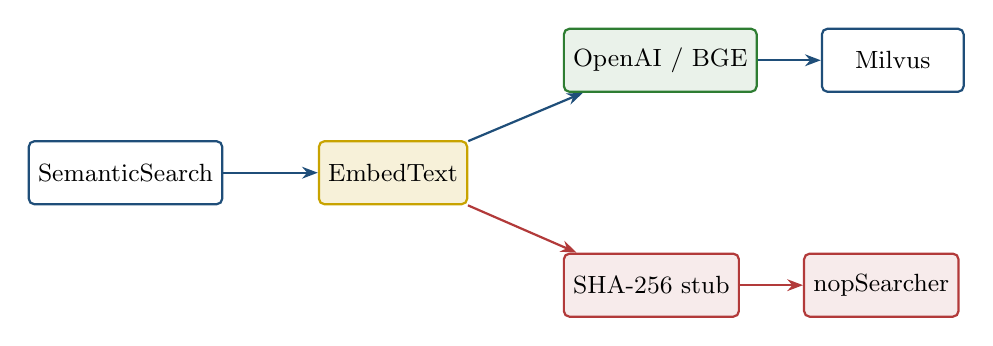
\begin{tikzpicture}[node distance=6mm and 12mm]
  \node[node-box]                            (s)   {SemanticSearch};
  \node[node-box,right=of s,node-warn]       (em)  {EmbedText};
  \node[node-box,above right=of em,node-ok]  (api) {OpenAI / BGE};
  \node[node-box,below right=of em,node-bad] (stub){SHA-256 stub};
  \node[node-box,right=8mm of api]           (mv)  {Milvus};
  \node[node-box,right=8mm of stub,node-bad] (nop) {nopSearcher};
  \draw[arrow] (s)  -- (em);
  \draw[arrow] (em) -- (api);
  \draw[arrow-bad] (em) -- (stub);
  \draw[arrow] (api) -- (mv);
  \draw[arrow-bad] (stub) -- (nop);
\end{tikzpicture}
\vspace{1mm}
\small
\begin{itemize}
  \item \texttt{EMBEDDING\_API\_URL} 未配 $\to$ SHA-256 stub 兜底；上线节奏 OpenAI $\to$ BGE 省 token；dim=768 硬约束。
  \item Milvus 走 \texttt{MilvusSearcher} 接口，未注入 $\to$ nop 返回 nil $\to$ hybrid 退化为纯 ES。
  \item \textbf{Milvus 挂只丢语义，关键词召回不受影响}。
\end{itemize}
\end{frame}

\begin{frame}[shrink]{HNSW 的三个核心参数（业务旋钮）}
\begin{tabular}{@{}lll@{}}
\toprule
参数              & 含义                             & gomall 当前值 \\
\midrule
\texttt{M}        & 节点最大邻居数                   & 16            \\
\texttt{efConstruction} & 建图时候选池大小            & 200           \\
\texttt{efSearch} & 查询时候选池大小                 & 64            \\
\bottomrule
\end{tabular}
\vspace{2mm}
\begin{itemize}
  \item \texttt{M} 大 $\to$ 图更密集，召回更准，但内存涨。常见 16--48。
  \item \texttt{efConstruction} 大 $\to$ 建图更慢但更优，回填速度敏感场景调低。
  \item \texttt{efSearch} 大 $\to$ 召回更准延迟更高，是\textbf{查询时}唯一可调旋钮 —— SRE 故障时的\textbf{减压阀}。
\end{itemize}
\end{frame}

\begin{frame}[fragile,shrink]{代码段 5：HNSW 索引建立 + 查询参数}
\begin{lstlisting}[language=Go,firstnumber=80,basicstyle=\ttfamily\tiny]
// 建索引：M=16, efConstruction=200
idx, _ := entity.NewIndexHNSW(entity.L2, hnswM, hnswEfConstruction)
existing, _ := MilvusClient.DescribeIndex(ctx, ProductVectorCollection,
    productVectorVectorField)
if len(existing) == 0 {
    MilvusClient.CreateIndex(ctx, ProductVectorCollection,
        productVectorVectorField, idx, false)
}
MilvusClient.LoadCollection(ctx, ProductVectorCollection, false)

// 查询：efSearch=64
sp, _ := entity.NewIndexHNSWSearchParam(hnswEfSearch)
results, _ := MilvusClient.Search(ctx, ProductVectorCollection,
    []string{}, expr, []string{"id"},
    []entity.Vector{entity.FloatVector(queryVec)},
    "vector", entity.L2, topK, sp)
\end{lstlisting}
\end{frame}

\begin{frame}[shrink]{代码段 5 逐行讲解（业务对照）}
\begin{itemize}
  \item \textbf{L81}：\texttt{NewIndexHNSW(L2, M, efConstruction)} 决定索引结构；L2 是欧氏距离，与 BGE / text-embedding-3 默认归一化向量兼容。
  \item \textbf{L82--87}：先 \texttt{DescribeIndex} 判断有没有索引，\textbf{没有才建}。EnsureProductVectorCollection 幂等，重启不会重建 —— SRE 安心运维。
  \item \textbf{L88}：\texttt{LoadCollection} 让 collection 进入内存。HNSW 索引\textbf{in-memory}，没 load 就不能查。
  \item \textbf{L91--96}：\texttt{NewIndexHNSWSearchParam(efSearch)} 是\textbf{查询时}调旋钮 —— 不用重建索引就能调召回精度/延迟权衡。
  \item \textbf{业务对应}：efSearch 是 SRE 故障时的\textbf{减压阀}，告警来了先调小，召回准确性损 1\%--3\% 换 P95 减半。
\end{itemize}
\end{frame}

% ============================================================
\section{客服话术：三个真实客诉怎么答}
% ============================================================

\begin{frame}[shrink]{客诉案例 1：用户搜不到 + 客服话术}
\textbf{用户原话}："我搜'蓝牙耳机'一个都没有，你们是不是没货？"
\vspace{2mm}
\begin{itemize}
  \item \textbf{后台排查 (30s)}：进 admin 后台搜同词 $\to$ 看是否走 ES / 走 LIKE。
  \item \textbf{若 ES 全挂}：业务码无（HTTP 200），监控 \texttt{search\_es\_fallback\_total}。
  \item \textbf{客服回复模板}："您看到的是降级结果，搜索系统正在抢修，30 分钟内恢复。您可以按类目浏览。"
  \item \textbf{若 ES 正常但 0 命中}：检查类目过滤是否锁死、检查"蓝牙"是否被分词器分错。
  \item \textbf{客服回复模板}："您可以试试'无线耳机'或具体品牌名，系统会推荐更相关的商品。"
\end{itemize}
\end{frame}

\begin{frame}[shrink]{客诉案例 2：商家"我上架了为什么搜不到" + 客服话术}
\textbf{商家原话}："我刚上架的 SKU 12345，搜不到，是不是上架失败？"
\vspace{2mm}
\begin{itemize}
  \item \textbf{后台排查 (1min)}：查 \texttt{product} 表 SKU 12345 存在 $\to$ 上架\textbf{未失败}。
  \item \textbf{排查 outbox}：查 \texttt{outbox} 表对应 product\_id 的 \texttt{product.changed} 行 status：
        \begin{itemize}\item \texttt{pending} 5min 内 $\to$ 正在同步，等就好\item \texttt{pending} \textgreater 5min $\to$ Publisher 卡住 / RMQ 不通\item \texttt{sent} 但 ES 无 $\to$ Indexer 报错或 ES 拒收\end{itemize}
  \item \textbf{客服回复模板}："上架已成功，搜索索引同步中，预计 5 分钟内可搜。如超时请回复我们。"
  \item \textbf{兜底操作}：调 \texttt{admin/search/backfill} 直接灌一次 ES。
\end{itemize}
\end{frame}

\begin{frame}[shrink]{客诉案例 3：用户搜到下架商品 + 客服话术}
\textbf{用户原话}："我搜到一个商品点进去显示已下架，是不是骗人？"
\vspace{2mm}
\begin{itemize}
  \item \textbf{根因}：商家下架 $\to$ DB \texttt{on\_sale=false} $\to$ \textbf{outbox 事件未投递 / Indexer 漏消费} $\to$ ES 里 \texttt{on\_sale=true} 仍在召回。
  \item \textbf{后台排查 (1min)}：DB \texttt{on\_sale} 与 ES doc 字段对比，不一致即定位。
  \item \textbf{业务码}：无（HTTP 200，命中后端再过滤）。
  \item \textbf{客服回复模板}："该商品已下架，搜索结果尚在更新，5 分钟内会消失。给您带来困扰，赠送 5 元无门槛券。"
  \item \textbf{兜底操作}：手动 \texttt{DeleteProduct(ID)} 删除 ES 文档；事后补 backfill。
  \item \textbf{长期方案}：搜索结果在返回 client 前\textbf{再过一遍 DB} 校验 on\_sale —— 牺牲 5ms 延迟换 0 客诉。
\end{itemize}
\end{frame}

% ============================================================
\section{业务边界、容量与个性化路线图}
% ============================================================

\begin{frame}[shrink]{业务边界：本搜索不做什么（诚实清单）}
\begin{itemize}
  \item \textbf{无同义词字典}：分词靠 standard analyzer，\textbf{未装 IK 与同义词包} —— "苹果手机"靠向量召回兜，不靠词典。
  \item \textbf{无搜索历史}：用户搜过什么不存，无"最近搜索"功能。
  \item \textbf{无 trending 词}：首页搜索框无热词推荐，无"大家都在搜"。
  \item \textbf{无搜索建议（suggest）}：输入框不联想，无前缀补全。
  \item \textbf{无商家 SEO 自助调权重}：商家不能自己买"高权重位置"，所有商品按 BM25 + name\^{}3 公平排。
  \item \textbf{无个性化排序}：用户画像 / 历史点击 / 协同信号挂载点已留，\textbf{特征工程链路未接}。
  \item \textbf{无以图搜图}：CLIP / SigLIP 路线图阶段。
\end{itemize}
\keypoint{这些"不做"列出来不是甩锅，是\textbf{划清当前能力边界} —— 后续每接一条都要走 PRD + A/B。}
\end{frame}

\begin{frame}[shrink]{个性化排序路线图：三类特征 + 挂载点}
\begin{tabular}{@{}lll@{}}
\toprule
特征类      & 例子                          & 来源                  \\
\midrule
用户画像    & 性别 / 年龄段 / 价格带偏好   & user profile 表       \\
历史点击    & 7 天内点过的类目 / 品牌       & 点击日志 + 实时流     \\
协同信号    & 同类用户买过什么             & 离线 i2i / u2i 矩阵   \\
\bottomrule
\end{tabular}
\vspace{2mm}
\begin{itemize}
  \item 历史点击走"近因衰减" \texttt{exp(-(now-ts)/\(\tau\))}，\(\tau\) 取 3--7 天。
  \item \textbf{挂载点}：\texttt{h.Score += wPersonal * personalScore(uid, h.Product)}，加在融合分外面。
  \item Redis miss 走默认 0（保中性），永远比"用户画像污染基线"安全。
\end{itemize}
\end{frame}

\begin{frame}[shrink]{容量规划：1M / 10M / 100M SKU}
\begin{tabular}{@{}llll@{}}
\toprule
量级    & ES 节点         & Milvus 内存        & 索引重建时长   \\
\midrule
1M     & 1 node (4C8G)  & 4 GB (HNSW)        & 30 min        \\
10M    & 3 nodes (8C16G) & 32 GB (HNSW)      & 4 h           \\
100M   & 5+ nodes (16C32G) & 256 GB / 切 IVF\_PQ & 24 h+         \\
\bottomrule
\end{tabular}
\vspace{2mm}
\begin{itemize}
  \item gomall 当前 \textbf{956K} SKU，落在 1M 档，单节点足够。
  \item 10M 是分水岭：ES 必须分片 + 副本；HNSW 内存接近 32 GB 拐点。
  \item 100M 切 IVF\_PQ 量化索引，召回率换内存；同时考虑冷热分层。
\end{itemize}
\end{frame}

\begin{frame}[shrink]{以图搜图路线图 (CLIP / SigLIP)}
\begin{tikzpicture}[node distance=5mm and 10mm]
  \node[node-box]                            (img) {上传图片};
  \node[node-box,right=of img,node-warn]     (clip){CLIP / SigLIP\\image encoder};
  \node[node-box,right=of clip,node-ok]      (mv)  {Milvus\\image\_vector};
  \node[node-box,below=of mv]                (out) {Top-K\\相似商品};
  \node[node-box,below=of clip,node-warn]    (cat) {商品图\\离线编码};
  \draw[arrow] (img) -- (clip);
  \draw[arrow] (clip) -- (mv);
  \draw[arrow] (cat) -- (mv);
  \draw[arrow] (mv) -- (out);
\end{tikzpicture}
\vspace{2mm}
\begin{itemize}
  \item CLIP / SigLIP 把图片和文本映射到同一向量空间，可做"图找图"+"文找图"。
  \item 落地：另建 \texttt{image\_vector} collection（dim=512/768），与文本 collection 解耦。
  \item 商品图离线批量编码，写入走相同 outbox 路由，复用 indexer 模式。
\end{itemize}
\end{frame}

% ============================================================
\section{业务侧总结：四角色 KPI 全打通}
% ============================================================

\begin{frame}[shrink]{一张表把这套搜索系统讲完}
\begin{tabular}{@{}lll@{}}
\toprule
能力        & 实现                              & 代码位置                              \\
\midrule
关键词召回  & ES \texttt{multi\_match}           & repository/es/product\_index.go     \\
增量索引    & outbox $\to$ MQ $\to$ indexer     & service/search/indexer.go            \\
DB 兜底     & ES 客户端为 nil $\to$ LIKE        & service/search/product\_query.go:15 \\
全量回填    & admin 触发的 Backfill             & service/search/backfill.go           \\
语义召回    & Milvus + embedding                & service/search/semantic.go          \\
模型切换    & env: \texttt{EMBEDDING\_API\_URL}  & service/search/embedding.go          \\
启动静默    & defer recover                     & cmd/main.go:69--78                   \\
\bottomrule
\end{tabular}
\vspace{2mm}
\end{frame}

\begin{frame}[shrink]{四方视角 + 压测数据复核}
\begin{itemize}
  \item \textbf{C 端}：hybrid 召回 90\%+，自然语言搜得到，p95 < 200ms。
  \item \textbf{商家}：上架 5min 内可搜，outbox 解耦 = 上架本身永远不挂。
  \item \textbf{运营}：\texttt{name\^{}3} 字段加权 / 融合权重 / function\_score 三档旋钮齐备。
  \item \textbf{客服 / SRE}：ES / Milvus / Embedding 三档降级，主流程永不 5xx。
  \item 同库 PK 查询能跑 \textbf{62{,}226 RPS / p95 3ms} (product/show)，证明慢的是\textbf{查询类型}（LIKE / count），不是数据库本身。
  \item 对照 \texttt{/product/list} 全表 count 实测 \textbf{24.5 RPS / p95 2.50s}，印证"搜索搬到 ES"是必选项。
\end{itemize}
\vspace{1mm}
\keypoint{副本系统判据：\textbf{副本旧一点点不要命，副本错乱才要命}。outbox 把 "上架成功" 和 "可搜" 解耦，是 5min SLA 的工程根据。}
\end{frame}

% ============================================================
\appendix
% ============================================================

\begin{frame}[shrink]{面试 Q\&A (1/3)}
\textbf{Q1}：为什么不让上架 API 直接写 ES，而要 outbox？\\
\hspace{4mm}\small A：DB 与 ES 不同事务，同步写要么失败回滚（伤体验），要么不一致（伤召回）。outbox 把"DB 写成功" 和 "ES 写成功" 两件事拆开，分别保证。代码：

\vspace{2mm}
\textbf{Q2}：ES 挂掉，搜索接口为什么不直接 5xx？\\
\hspace{4mm}\small A：搜索是入口，5xx 等于 app 崩页。LIKE 慢一点也比白屏强 —— 业务承诺"搜索框永远可用"。代码：

\vspace{2mm}
\textbf{Q3}：hybrid 50/50 这个权重你怎么调？\\
\hspace{4mm}\small A：业务值，不是技术值。先 50/50 跑一轮，A/B 观察 CTR / 转化。短 query 偏关键词，长 query 偏语义。代码：

\vspace{2mm}
\textbf{Q4}：商家说"上架后 10 分钟还搜不到"，怎么定位？\\
\hspace{4mm}\small A：四步走：查 product 表确认入库 $\to$ 查 outbox 行 status $\to$ 查 RMQ 队列深度 $\to$ 查 ES doc。每步对应一个客服话术（见客诉案例 2）。代码：
\end{frame}

\begin{frame}[shrink]{面试 Q\&A (2/3)}
\textbf{Q5}：min-max 归一在什么场景会失效？\\
\hspace{4mm}\small A：所有分数等值时 span=0。代码里返回常量 1，意味着"两路一样可信"，让另一路决定排序。代码：

\vspace{2mm}
\textbf{Q6}：HNSW 的 efSearch 你怎么调？\\
\hspace{4mm}\small A：efSearch 是查询时旋钮，不用重建索引。延迟告警时调小（64$\to$32）召回率损 1\%--3\%，P95 减半。代码：

\vspace{2mm}
\textbf{Q7}：Milvus 挂了怎么办？为什么不直接 5xx？\\
\hspace{4mm}\small A：nopMilvusSearcher 返回空，hybrid 退化为纯 ES。关键词召回不受影响，只丢自然语言长尾。代码：

\vspace{2mm}
\textbf{Q8}：搜索结果命中下架商品（客诉案例 3）根因有几种？\\
\hspace{4mm}\small A：三种：DB 改 \texttt{on\_sale} 但 outbox 漏写、outbox 写了但 indexer 没消费、indexer 调 DeleteProduct 但 ES 拒收。长期方案：返回前再过一次 DB 校验。代码：
\end{frame}

\begin{frame}[shrink]{面试 Q\&A (3/3)}
\textbf{Q9}：5 分钟新鲜度 SLA 在哪一步可能掉？\\
\hspace{4mm}\small A：堆积一般出现在 RMQ 与 indexer 之间，Qos=32 + ES refresh\_interval=1s 下 p95 < 30s。监控 \texttt{search.product.indexer} queue\_depth。代码：

\vspace{2mm}
\textbf{Q10}：100M SKU 时这个架构还能用吗？\\
\hspace{4mm}\small A：ES 切多分片 + 副本；HNSW 内存撑不住改 IVF\_PQ 量化；冷热分层把老 SKU 放冷索引。

\vspace{2mm}
\textbf{Q11}：为什么不接同义词字典 / 搜索历史 / trending？\\
\hspace{4mm}\small A：业务边界。当前流量没到拐点，同义词靠 hybrid 向量召回兜，搜索历史涉及用户隐私单独立项，trending 词运营手动维护轮播。详见"业务边界"帧。

\vspace{2mm}
\textbf{Q12}：mapping 改了字段类型怎么办？\\
\hspace{4mm}\small A：ES mapping 字段类型不能原地改，必须 \texttt{reindex} 或新建索引 + alias 切换。回填走 admin/search/backfill。
\end{frame}

\begin{frame}[shrink]{代码位置总览 + 配套材料}
\footnotesize
\begin{description}
  \item[搜索 / 语义入口]
  \item[ES 检索 + mapping]
  \item[outbox 事件]
  \item[indexer 消费]
  \item[ES 兜底分支]
  \item[全量回填]
  \item[hybrid 融合 + embedding]
  \item[Milvus HNSW]
  \item[Milvus 接口抽象]
  \item[启动静默]
  \item[业务码表]
\end{description}
\vspace{2mm}
\small \textbf{配套}：deck 04 outbox / saga；deck 10 流量治理与降级；deck 11 一致性；stressTest/REPORT.md；docs/blog/10-milvus-vector-search.md；docs/blog/11-semantic-search.md。
\end{frame}

\end{document}
